\documentclass[a4paper, 11pt]{report}

% %%%
% Camp 100 Long Form Document Preamble
% %%%

% basic document setup
\usepackage{geometry}
\geometry{
a4paper,
total={170mm,257mm},
left=20mm,
top=20mm,
}
\usepackage[skip=0.7em]{parskip} % put in nice paragraph breaksq
\setlength\parindent{0pt} % get rid of the indent
\setcounter{tocdepth}{0} % set toc depth to only show chapters
\setcounter{secnumdepth}{3} % use section numbering for everything up too and including subsubsection

% remove hyphenation at end of line
\tolerance=1
\emergencystretch=\maxdimen
\hyphenpenalty=10000
\hbadness=10000

% document global variables, defined for all documents and used to fill blanks etc
% this comes at the top of the doc as we use these values throughout the entire preamble
% we also set here the language settings for the backpage of the document as it's easier to declare this as a global variable
\newcommand{\documentsetup}[6]{%
    \def\documentTitle{#1}
    \def\documentSubtitle{#2}
    \def\publishDate{#3}
    \def\documentID{#4}
    \def\documentLanguage{#5} % ISO 639 compliant 2 letter language code
    \def\documentStatus{#6}

    \ifthenelse{\equal{#5}{en}}{
        \def\backPageCampInfo{Camp 100, a project by Woodcraft Folk will bring together members of all ages from across the UK to camp together and live by the Woodcraft Folk values for a week in the summer of 2025. The camp celebrates Woodcraft Folk's 100th birthday and will celebrate it's past century while looking forward to the next 100 years.}
        \def\backPageWcfInfo{Woodcraft Folk is a registered charity in England \& Wales (1148195) and in Scotland (SC039791), and a limited company, registered in England \& Wales (8133727). Registered office: Holyoake House, Hanover Street, Manchester M60 0AS}
        \def\backPageCampSocials{Find Camp 100 on the internet}
        \def\backPageWcfSocials{Find Woodcraft Folk online}
    }%
    {}% false
    \ifthenelse{\equal{#5}{fr}}{
        \usepackage[french]{babel}
        \def\backPageCampInfo{Camp-French}
        \def\backPageWcfInfo{Wcf-French}
        \def\backPageCampSocials{fr}
        \def\backPageWcfSocials{fr}
    }%
    {}% false
    \ifthenelse{\equal{#5}{es}}{
        \def\backPageCampInfo{Camp-Spanish}
        \def\backPageWcfInfo{Wcf-Spanish}
        \def\backPageCampSocials{es}
        \def\backPageWcfSocials{es}
    }%
    {}% false
}



% packages for general use
\usepackage[dvipsnames, table]{xcolor}
\usepackage{graphicx}

\usepackage{tikz}
\usetikzlibrary{calc, shapes.callouts}
\usepackage{adjustbox}
\usepackage{fontawesome}
\usepackage{enumitem}
\usepackage{datetime2}
\usepackage{hyperref}
\usepackage{lastpage}
\usepackage{tcolorbox}
\usepackage{ifthen}
\usepackage{multicol}
\usepackage{multirow}
\usepackage{longtable}
\usepackage{ragged2e}
\usepackage{float}


% configure hyperref to do links & PDF metadata
\hypersetup{
    linktoc=none,
    pdfborderstyle={/S/U/W 1},
    colorlinks=false,
    allbordercolors=blue,
    breaklinks=true,
}
% these ones come in a different block as they must be dealt with at the start of the document
\makeatletter
\AtBeginDocument{
  \hypersetup{
    pdftitle={ \documentTitle },
    pdfauthor={Camp 100},
    pdfsubject={ \documentSubtitle },
    pdfcreator={LaTeX}
  }
}
\makeatother
% redefine \href so it uses text color blue to make links more obvious
\let\oldhref\href
\renewcommand{\href}[2]{\oldhref{#1}{\textcolor{blue}{#2}}}

\newcommand{\internallink}[2]{\hyperref[#1]{\textcolor{blue}{#2}}}


%% COLORS
\definecolor{wcf-accent}{HTML}{6d8f41}
\definecolor{c100-red}{HTML}{F04C58}
\definecolor{c100-green}{HTML}{087F5C}
\definecolor{c100-beige}{HTML}{E9E1CA}
\definecolor{c100-orange}{HTML}{EC7E2C}
\definecolor{c100-grey}{HTML}{545454}

% setup setup fonts
% we manually specify to use the `_Light_Oblique' varient of Quicksand for italics as the font doesn't include an italic face by default.
\usepackage{fontspec}
\setmainfont[Ligatures=TeX, ItalicFont=*_Light_Oblique]{Quicksand}
\setsansfont[Ligatures=TeX, ItalicFont=*_Light_Oblique]{Quicksand}

% tables
\renewcommand{\arraystretch}{1.6} % make cells vertically bigger

\newcommand{\tablehead}[1]{\centering\arraybackslash \cellcolor{c100-grey}\leavevmode\color{white}\textbf{#1}} % we try this as it actually allows automatic linebreaks in the headings
% \newcommand{\tablehead}[1]{\multicolumn{1}{c}{\cellcolor{c100-red}\textcolor{white}{\textbf{#1}}}}



% Document Title Page
% adapted from: https://www.reddit.com/r/LaTeX/comments/faij1n/my_first_cover_page_done_in_latex_is_it/
\newcommand{\makedocumenttitlepage}{\begin{titlepage}
    \begin{tikzpicture}[overlay,remember picture]

        % \fill[black!2] (current page.south west) rectangle (current page.north east);
        
        % line 01
        \begin{scope}[transform canvas ={rotate around ={45:($(current page.north west)+(-.5,-6)$)}}]
        \shade[rounded corners=18pt, left color=c100-orange, right color=c100-orange] ($(current page.north west)+(-.5,-6)$) rectangle ++(9,1.5);
        \end{scope}
        
        % line 02
        \begin{scope}[transform canvas ={rotate around ={45:($(current page.north west)+(.5,-10)$)}}]
        \shade[rounded corners=18pt, left color=c100-green ,right color=c100-green] ($(current page.north west)+(0.5,-10)$) rectangle ++(15,1.5);
        \end{scope}
        
        % line 03
        \begin{scope}[transform canvas ={rotate around ={45:($(current page.north)+(-1.5,-3)$)}}]
        \shade[rounded corners=12pt, left color=c100-grey, right color=c100-grey] ($(current page.north)+(-1.5,-3)$) rectangle ++(9,0.8);
        \end{scope}
        
        % line 04
        \begin{scope}[transform canvas ={rotate around ={45:($(current page.north)+(-3,-8)$)}}]
        \shade[rounded corners=28pt, left color=c100-red, right color=c100-red] ($(current page.north)+(-3,-8)$) rectangle ++(15,1.8);
        \end{scope}
        
        % line 05
        \begin{scope}[transform canvas ={rotate around ={45:($(current page.north west)+(4,-15.5)$)}}]
        \shade[rounded corners=25pt, left color=c100-green, right color=c100-green] ($(current page.north west)+(4,-15.5)$) rectangle ++(30,1.8);
        \end{scope}
        
        % line 06
        \begin{scope}[transform canvas ={rotate around ={45:($(current page.north west)+(13,-10)$)}},]
        \shade[rounded corners=22pt, left color=c100-orange,right color=c100-orange] ($(current page.north west)+(13,-10)$) rectangle ++(15,1.5);
        \end{scope}
        
        % line 07
        \begin{scope}[transform canvas ={rotate around ={45:($(current page.north west)+(19,-5.65)$)}},]
        \shade[rounded corners=12pt, left color=c100-grey,right color=c100-grey] ($(current page.north west)+(19,-5.65)$) rectangle ++(15,0.8);
        \end{scope}
        
        % line 08
        \begin{scope}[transform canvas ={rotate around ={45:($(current page.north west)+(18,-8)$)}},]
        \shade[rounded corners=8pt, left color=c100-green,right color=c100-green] ($(current page.north west)+(18,-8)$) rectangle ++(15,0.6);
        \end{scope}
        
        % line 09
        \begin{scope}[transform canvas ={rotate around ={45:($(current page.north west)+(20,-9)$)}}]
        \shade[rounded corners=20pt, left color=c100-red, right color=c100-red] ($(current page.north west)+(20,-9)$) rectangle ++(14,1.2);
        \end{scope}
        
        \node[inner sep=0pt] () at ($(current page.center)+(5,-11)$){
\includegraphics[width=0.45\textwidth]{../global-logo-c100-wide.png}};
        \node[inner sep=0pt] () at ($(current page.center)+(-5,-11)$){
\includegraphics[width=0.45\textwidth]{../global-logo-wcf-wide.png}};
        
        \node[text width=\textwidth,align=center] at ($(current page.center)+(0,-3.5)$) {{\Huge \documentTitle}};
        
        \node[text width=\textwidth,align=center] at ($(current page.center)+(0,-5.5)$) {{\Large{\textit{\documentSubtitle}}} \\[2em] \large \publishDate};
        
        \end{tikzpicture}
\end{titlepage}
}

% Document Back Page
\newcommand{\makedocumentbackpage}{\newpage
  \thispagestyle{empty}
  \begin{tikzpicture}[overlay,remember picture]

      % \fill[black!2] (current page.south west) rectangle (current page.north east);
      
      % line 01
      \begin{scope}[transform canvas ={rotate around ={45:($(current page.north west)+(-.5,-6)$)}}]
      \shade[rounded corners=18pt, left color=c100-orange, right color=c100-orange] ($(current page.north west)+(-.5,-6)$) rectangle ++(9,1.5);
      \end{scope}
      
      % line 02
      \begin{scope}[transform canvas ={rotate around ={45:($(current page.north west)+(.5,-10)$)}}]
      \shade[rounded corners=18pt, left color=c100-green ,right color=c100-green] ($(current page.north west)+(0.5,-10)$) rectangle ++(15,1.5);
      \end{scope}
      
      % line 03
      \begin{scope}[transform canvas ={rotate around ={45:($(current page.north)+(-1.5,-3)$)}}]
      \shade[rounded corners=12pt, left color=c100-grey, right color=c100-grey] ($(current page.north)+(-1.5,-3)$) rectangle ++(9,0.8);
      \end{scope}
      
      % line 04
      \begin{scope}[transform canvas ={rotate around ={45:($(current page.north)+(-3,-8)$)}}]
      \shade[rounded corners=28pt, left color=c100-red, right color=c100-red] ($(current page.north)+(-3,-8)$) rectangle ++(15,1.8);
      \end{scope}
      
      % line 05
      \begin{scope}[transform canvas ={rotate around ={45:($(current page.north west)+(4,-15.5)$)}}]
      \shade[rounded corners=25pt, left color=c100-green, right color=c100-green] ($(current page.north west)+(4,-15.5)$) rectangle ++(30,1.8);
      \end{scope}
      
      % line 06
      \begin{scope}[transform canvas ={rotate around ={45:($(current page.north west)+(13,-10)$)}},]
      \shade[rounded corners=22pt, left color=c100-orange,right color=c100-orange] ($(current page.north west)+(13,-10)$) rectangle ++(15,1.5);
      \end{scope}
      
      % line 07
      \begin{scope}[transform canvas ={rotate around ={45:($(current page.north west)+(19,-5.65)$)}},]
      \shade[rounded corners=12pt, left color=c100-grey,right color=c100-grey] ($(current page.north west)+(19,-5.65)$) rectangle ++(15,0.8);
      \end{scope}
      
      % line 08
      \begin{scope}[transform canvas ={rotate around ={45:($(current page.north west)+(18,-8)$)}},]
      \shade[rounded corners=8pt, left color=c100-green,right color=c100-green] ($(current page.north west)+(18,-8)$) rectangle ++(15,0.6);
      \end{scope}
      
      % line 09
      \begin{scope}[transform canvas ={rotate around ={45:($(current page.north west)+(20,-9)$)}}]
      \shade[rounded corners=20pt, left color=c100-red, right color=c100-red] ($(current page.north west)+(20,-9)$) rectangle ++(14,1.2);
      \end{scope}

    \end{tikzpicture}
      
    % textual boxes at the bottom of the page
    \begin{tikzpicture}[overlay,remember picture]
      % top left box, textual information about C100
      \node[rectangle, anchor=north west,
              rounded corners=18pt,inner sep=11pt,
              fill=c100-green,
              minimum height=11em] () at
              ($(current page.center)+(-9, -3)$)
              {\parbox[t]{0.55\textwidth}{\color{white} \backPageCampInfo}};

      % top right box, social media contact for C100
      \node[rectangle, anchor=north west,
              rounded corners=18pt,inner sep=11pt,
              fill=c100-red,
              minimum height=11em] () at
              ($(current page.center)+(2,-3)$)
              {\parbox[t]{0.35\textwidth}{\color{white} \backPageCampSocials\\[-0.5em] \begin{itemize}[leftmargin=1.5em]
                \setlength\itemsep{0.7em}
                \item[\faInstagram] camp100wcf
                \item[\faFacebook] camp100wcf
                \item[\faLink] camp100.org.uk
              \end{itemize}}};
      
      % bottom left box, WCF charity disclaimer
      \node[rectangle, anchor=north west,
              rounded corners=18pt,inner sep=11pt,
              fill=c100-red,
              minimum height=11em] () at
              ($(current page.center)+(-9,-8)$)
              {\parbox[t]{0.4\textwidth}{\color{white} \backPageWcfInfo}};
      % bottom middle, WCF social media
      \node[rectangle, anchor=north west,
              rounded corners=18pt,inner sep=11pt,
              fill=c100-orange,
              minimum height=11em] () at
              ($(current page.center)+(-0.95,-8)$)
              {\parbox[t]{0.25\textwidth}{\color{white} \backPageWcfSocials\\[-0.5em] \begin{itemize}[leftmargin=1.5em]
                \setlength\itemsep{0.7em}
                \item[\faInstagram] woodcraftfolk
                \item[\faFacebook] woodcraftfolk
                \item[\faLink] woodcraft.org.uk
              \end{itemize}}};
      % bottom right box, WCF logo
      \node[rectangle, anchor=north west,
              rounded corners=18pt,inner sep=11pt,
              fill=c100-green,
              minimum height=11em] () at
              ($(current page.center)+(4.5,-8)$)
              {\parbox[t]{0.2\textwidth}{\color{white} 
\includegraphics[width=0.2\textwidth]{../global-logo-wcf-black.png}}};
      % very bottom line, document information
      \node[rectangle, anchor=north west,
              rounded corners=12pt,inner sep=11pt,
              fill=c100-grey] () at
              ($(current page.center)+(-9,-13)$)
              {\parbox[t]{0.99\textwidth}{\color{white} \footnotesize{\texttt{\documentID}\ (\texttt{\jobname .tex}) compiled at \texttt{\DTMnow}\ with version \texttt{\documentStatus} in language \texttt{\documentLanguage}}}};
    \end{tikzpicture}
  

}

% section titles
% chapter heading adapted from: https://texblog.net/latex-archive/uncategorized/fancy-chapter-tikz/
\usepackage[explicit]{titlesec}

% we only want to deal with chapters if document class is a report; as it'll break in articles otherwise
\makeatletter
\@ifclassloaded{report}{%
    \titlespacing*{\chapter}{0pt}{30pt}{60pt}

    \titleformat{\chapter}
    {\gdef\chapterlabel{}
    \normalfont\sffamily\Huge\bfseries}
    {\gdef\chapterlabel{\thechapter\ | }}{0pt}
    {\begin{tikzpicture}[remember picture,overlay]
        % line 01
        \begin{scope}[transform canvas ={rotate around ={45:($(current page.north west)+(13,-10)$)}},]
        \shade[rounded corners=12pt, left color=c100-grey,right color=c100-grey] ($(current page.north west)+(21,-7)$) rectangle ++(15,0.8);
        \end{scope}
        % line 02
        \begin{scope}[transform canvas ={rotate around ={45:($(current page.north west)+(13,-10)$)}},]
        \shade[rounded corners=20pt, left color=c100-red,right color=c100-red] ($(current page.north west)+(17,-9)$) rectangle ++(15,1.3);
        \end{scope}
        % line 03
        \begin{scope}[transform canvas ={rotate around ={45:($(current page.north west)+(19,-5.65)$)}},]
        \shade[rounded corners=12pt, left color=c100-orange,right color=c100-orange] ($(current page.north west)+(19,-5)$) rectangle ++(15,0.8);
        \end{scope}
        \node[anchor=west,yshift=1.5em, rectangle,
                rounded corners=18pt,inner sep=11pt,
                fill=c100-green] 
                {\parbox[t]{0.6\textwidth}{\color{white}\chapterlabel#1}};
    \end{tikzpicture}
    }
    % redefine \chapter so it uses pagestyle=fancy
    \makeatletter
    \renewcommand\chapter{\if@openright\cleardoublepage\else\clearpage\fi
    \thispagestyle{fancy}%
    \global\@topnum\z@
    \@afterindentfalse
    \secdef\@chapter\@schapter}
    \makeatother
}
\makeatother



\titleformat{\section}
    {\normalfont\LARGE\sffamily\bfseries\color{black}}
    {\tcbox[colback=c100-green, colframe=c100-green, coltext=white, on line, boxsep=0pt, left=4pt, right=4pt, top=4pt, bottom=4pt]{\thesection}}{0.2em}{#1}
\titleformat{\subsection}
    {\normalfont\Large\sffamily\bfseries\color{black}}
    {\tcbox[colback=c100-green, colframe=c100-green, coltext=white, on line, boxsep=0pt, left=4pt, right=4pt, top=4pt, bottom=4pt]{\thesubsection}}{0.2em}{#1}
\titleformat{\subsubsection}
    {\normalfont\large\sffamily\bfseries\color{black}}
    {\tcbox[colback=c100-green, colframe=c100-green, coltext=white, on line, boxsep=0pt, left=4pt, right=4pt, top=4pt, bottom=4pt]{\thesubsubsection}}{0.2em}{#1}




% headers and footers
\usepackage{fancyhdr}


\pagestyle{fancy}
\fancyhf{}
\fancyfoot[L]{\documentTitle}
\fancyfoot[C]{\textbf{\thepage}\ of \pageref*{LastPage}}
\fancyfoot[R]{\publishDate}
\renewcommand{\footrulewidth}{0.4pt}
\renewcommand{\headrulewidth}{0.0pt}
\addtolength{\topmargin}{-1.59999pt}
\setlength{\headheight}{13.59999pt}

% now we do headers and footers for non-release version watermarks
\AtBeginDocument{
    \usepackage{draftwatermark}
    \DraftwatermarkOptions{
        stamp=false,
        text={\documentStatus},
        color=red!30
    }
    \ifthenelse{\equal{\documentStatus}{proof}}{
        \DraftwatermarkOptions{stamp=true}
    }%
    {}% if not set to 1
    \ifthenelse{\equal{\documentStatus}{draft}}{
        \DraftwatermarkOptions{stamp=true}
    }%
    {}% if not set to 1

    
}

% callouts

\usepackage[framemethod=TikZ]{mdframed}
\mdfsetup{skipabove=\topskip,
skipbelow=\topskip,
leftmargin=0cm,
rightmargin=0cm,
linewidth=3pt
}

% Red callout
\mdfdefinestyle{callout-red}{%
linecolor=c100-red!70,
backgroundcolor=c100-red!10,
topline=false,
bottomline=false,
rightline=false,
frametitlebackgroundcolor=c100-red!30,
}
\newenvironment{callout-red}[1]
    {\begin{mdframed}[style=callout-red,frametitle={#1}]
        }
        {
    \end{mdframed}
    }

% Orange callout
\mdfdefinestyle{callout-orange}{%
linecolor=c100-orange!70,
backgroundcolor=c100-orange!10,
topline=false,
bottomline=false,
rightline=false,
frametitlebackgroundcolor=c100-orange!30,
}
\newenvironment{callout-orange}[1]
    {\begin{mdframed}[style=callout-orange,frametitle={#1}]
        }
        {
    \end{mdframed}
    }

% Green callout
\mdfdefinestyle{callout-green}{%
linecolor=c100-green!70,
backgroundcolor=c100-green!10,
topline=false,
bottomline=false,
rightline=false,
frametitlebackgroundcolor=c100-green!30,
}
\newenvironment{callout-green}[1]
    {\begin{mdframed}[style=callout-green,frametitle={#1}]
        }
        {
    \end{mdframed}
    }

% bold callouts - to be used sparingly

\mdfdefinestyle{bold-callout-generic}{
linewidth=0.0em,
fontcolor=white,
roundcorner=0.25em,
font=\bfseries
}
\newenvironment{callout-bold-green}
    {\begin{mdframed}[style=bold-callout-generic, backgroundcolor=c100-green]
        }
        {
    \end{mdframed}
    }
\newenvironment{callout-bold-orange}
    {\begin{mdframed}[style=bold-callout-generic, backgroundcolor=c100-orange]
        }
        {
    \end{mdframed}
    }
\newenvironment{callout-bold-red}
    {\begin{mdframed}[style=bold-callout-generic, backgroundcolor=c100-red]
        }
        {
    \end{mdframed}
    }


% TIKZ
\tikzset{
    c100-speech-callout/.style= {color = white,
                        draw,
                        shape=rectangle callout,
                        fill = c100-green,
                        rounded corners=0.25em,
                        line width = 0.1em,
                        inner xsep = 0.5em,
                        inner ysep = 0.5em,
                        callout relative pointer={(1.25cm,-1cm)},
                        callout pointer width=2cm,
                        font=\bfseries},
    c100-sc-left/.style= {callout relative pointer={(-1.25cm,-1cm)}}
}

% QR Codes
\usepackage{qrcode}
\usepackage{wrapfig}

\newcommand{\insertqrcode}[2]{%
\begin{wrapfigure}{r}{0.35\textwidth}
  \centering
  \begin{mdframed}[linecolor=c100-green, linewidth=0.2em, roundcorner=0.25em, skipabove=0em, skipbelow=0em]
    \begin{center}
      \qrcode[height=0.9\textwidth, nolinks, level=M, version=4]{#1}
      
      {\small \vspace{0.5em} \href{#1}{#2}}
    \end{center}
    
  \end{mdframed}
\end{wrapfigure}
}

\documentsetup{Booking Handbook}{Instructions for all things Bookings}{07 May 2025}{booking-handbook}{en}{v3}

\usepackage{pdfpages}

\begin{document}
\makedocumenttitlepage

\tableofcontents

\chapter{Introduction}
Welcome to the Booking Handbook, a guide to the booking process for Camp 100! We hope that this handbook will support groups and individuals who are booking into Camp 100 and be a walk-through guide to starting your journey to our centenary celebrations. 

\section{Booking System}
We will be using the Woodcraft Folk camp booking system for Camp 100 (this is a modified and updated version of what was used for Common Ground and Venturer Camp 2023). 

Information on how to access the booking system and how to use it are available in the subsequent sections of this handbook.

\section{Support}
If you need support with the booking process or have any questions which aren't answered in this guide, feel free to get in touch on info@camp100.org.uk .

\section{Overview of Booking Process}
The booking process has a number of parts.
\begin{enumerate}
    \item Apply to book \internallink{chap:apply}{(Section \ref*{chap:apply})}
    \item Book \internallink{chap:booking}{(Section \ref*{chap:booking})}
    \item Edit booking \internallink{chap:edit}{(Section \ref*{chap:edit})}
\end{enumerate}

\section{Individual Bookings}
Where possible, you should book as part of a group. If you are an individual who is planning to camp with a group you are part of or affiliated with, please get in contact with them to be included in their booking. If you would like to book as an individual DF or volunteer see below how to select individual booking in section 2. We have made it possible for individuals (and groups up to 3 people) to pay by card. 

\section{Woodcraft Folk Membership \& DBS}
Everyone over the age of 16 attending the camp from the UK will need to be a member of Woodcraft Folk. Information on how to become a member can be found on the Woodcraft Website \href{https://woodcraft.org.uk/get-involved/volunteering-with-woodcraft-folk/}{here}.

Woodcraft Folk members over the age of 16 taking on a role in which they are responsible for under 16 year olds, and everyone over the age of 18, will need to have completed a DBS/ PVG check. Information on how to do this will be available through your local Membership Secretary or through the \href{https://woodcraft.org.uk/get-involved/volunteering-with-woodcraft-folk/}{Woocraft Folk Website}.

Further information on Safeguarding at Camp 100 will be made available on our dedicated safeguarding webpage. 

\section{International Safeguarding}
International campers over the age of 18 will need to sign a safeguarding declaration form before attending Camp 100. This is to ensure we can keep all campers and volunteers as safe as possible during the event. International campers attending who are 16-18 taking on a volunteer role during the camp will also need to fill in the form. Once booked in you will receive an electronic copy of the form to the email address provided. 


\chapter{Stage 1: Apply To Book}
\label{chap:apply}
The first stage for booking is to apply to book. You will need to complete this stage in order to create a booking. Applying to book is not committing that your group will come, it is simply giving us an indication that you wish to do so and giving us an idea of numbers. Groups coming from outside of Western Europe will need to do this by \textbf{1st December 2024} so we can plan funding allocation (but we won't necessarily be able to fund every group who applies). After you have been approved to book, you will be able to login and edit your booking.

\begin{enumerate}
    \item Go to the \href{https://bookings.camp100.org.uk}{Camp 100 Booking System}
    \item Click log in to book.\\
    Next to the login button is a dark/light mode toggle. This will change the theme of the app to be either dark or light. For simplicity, all screenshots in this guide will be in light mode.
    \begin{figure}[H]
        \centering
        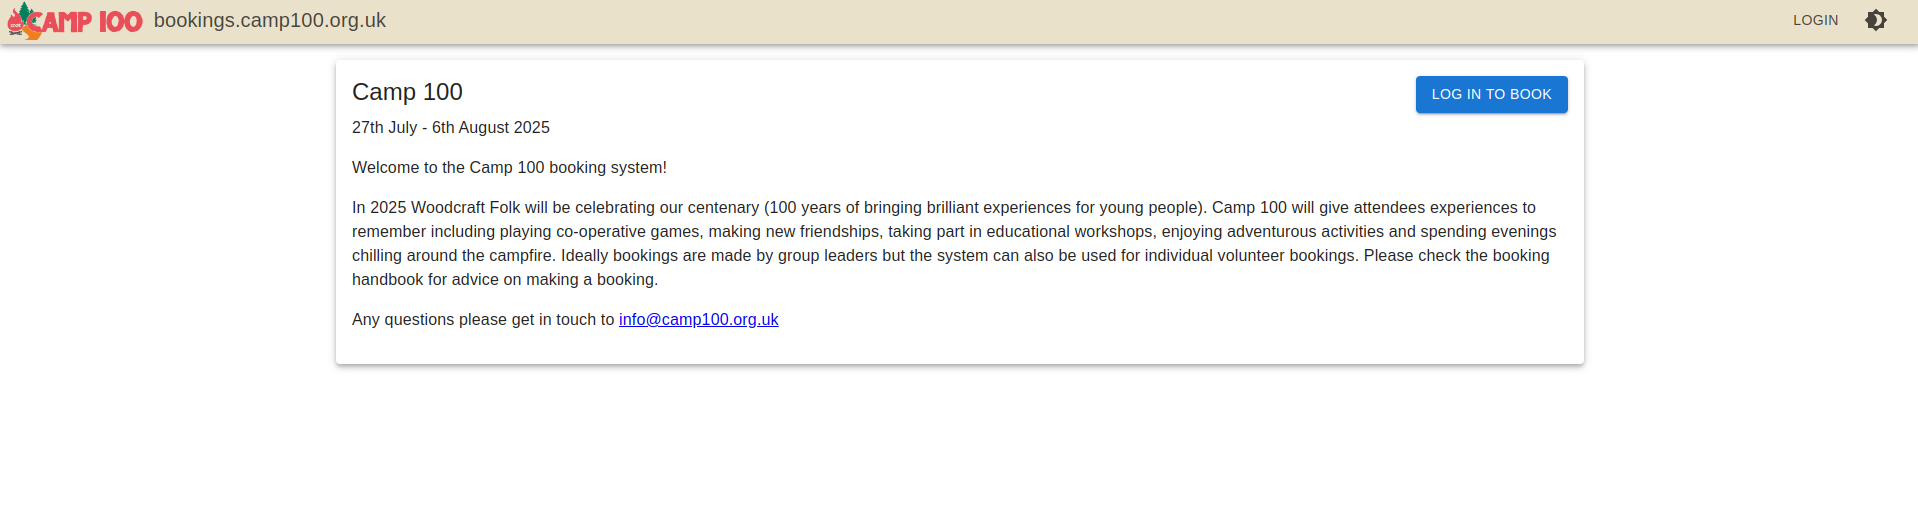
\includegraphics[width=0.9\textwidth]{assets/1-homepage.png}
        \caption{Booking System's Homepage}
    \end{figure}
    \item Select one of these methods to login
    \begin{figure}[H]
        \centering
        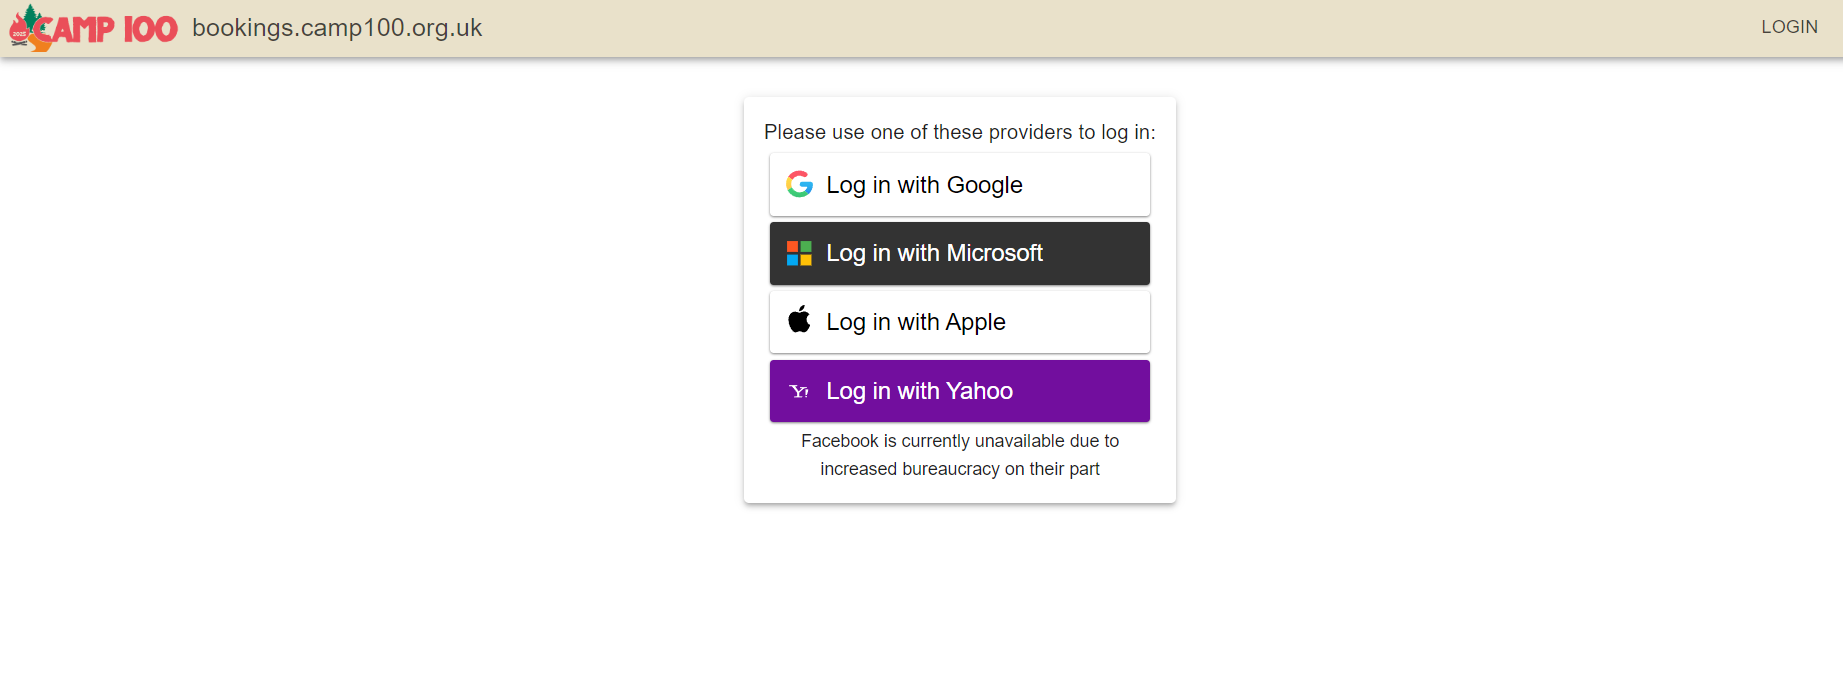
\includegraphics[width=0.9\textwidth]{assets/1-login.png}
        \caption{Login Options}
    \end{figure}
    \item Follow instructions on screen for how to login using your method of choice.
    \item When you have successfully logged in, you will be redirected to the screen below. Your (or the account you are using) name will appear in the top right corner. Enter your name and re-enter your email address, click save.
    \begin{figure}[H]
        \centering
        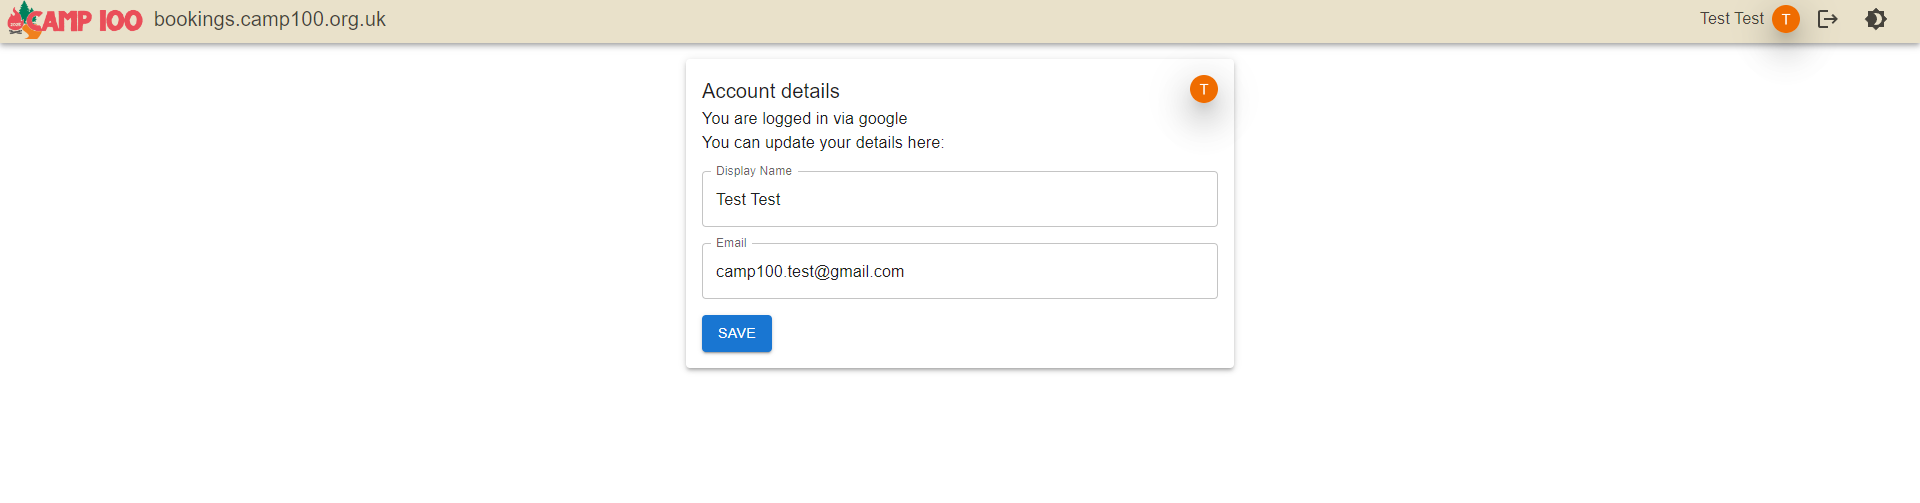
\includegraphics[width=0.9\textwidth]{assets/1-create-account.png}
        \caption{Create Account Options}
    \end{figure}
    \item You will be redirected to the home page. Click`apply to book'
    \begin{figure}[H]
        \centering
        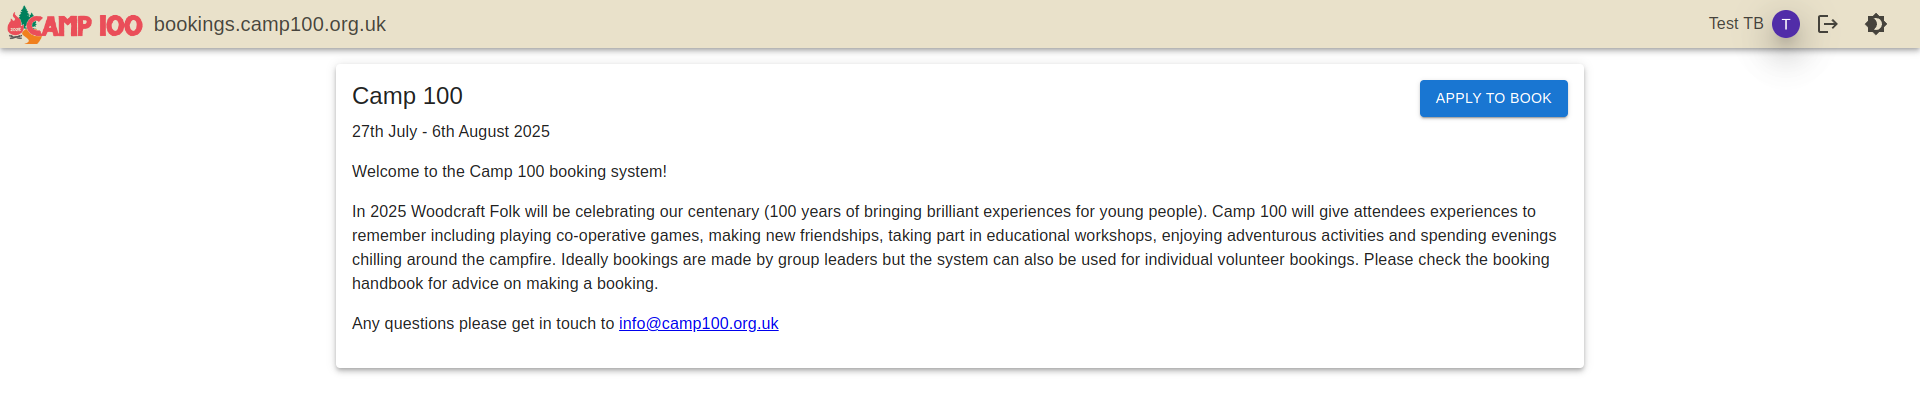
\includegraphics[width=0.9\textwidth]{assets/1-homepage-loggedin.png}
        \caption{Apply To Book button}
    \end{figure}
    \item Tick whether you are making a group or individual booking. You may need to re-enter your name and email. Select your organisation from the dropdown menu and enter the approximate number of people you are planning to bring into the textbox when prompted then press Submit. (Don't worry if this changes but an estimate is really helpful for us)
    \begin{figure}[H]
        \centering
        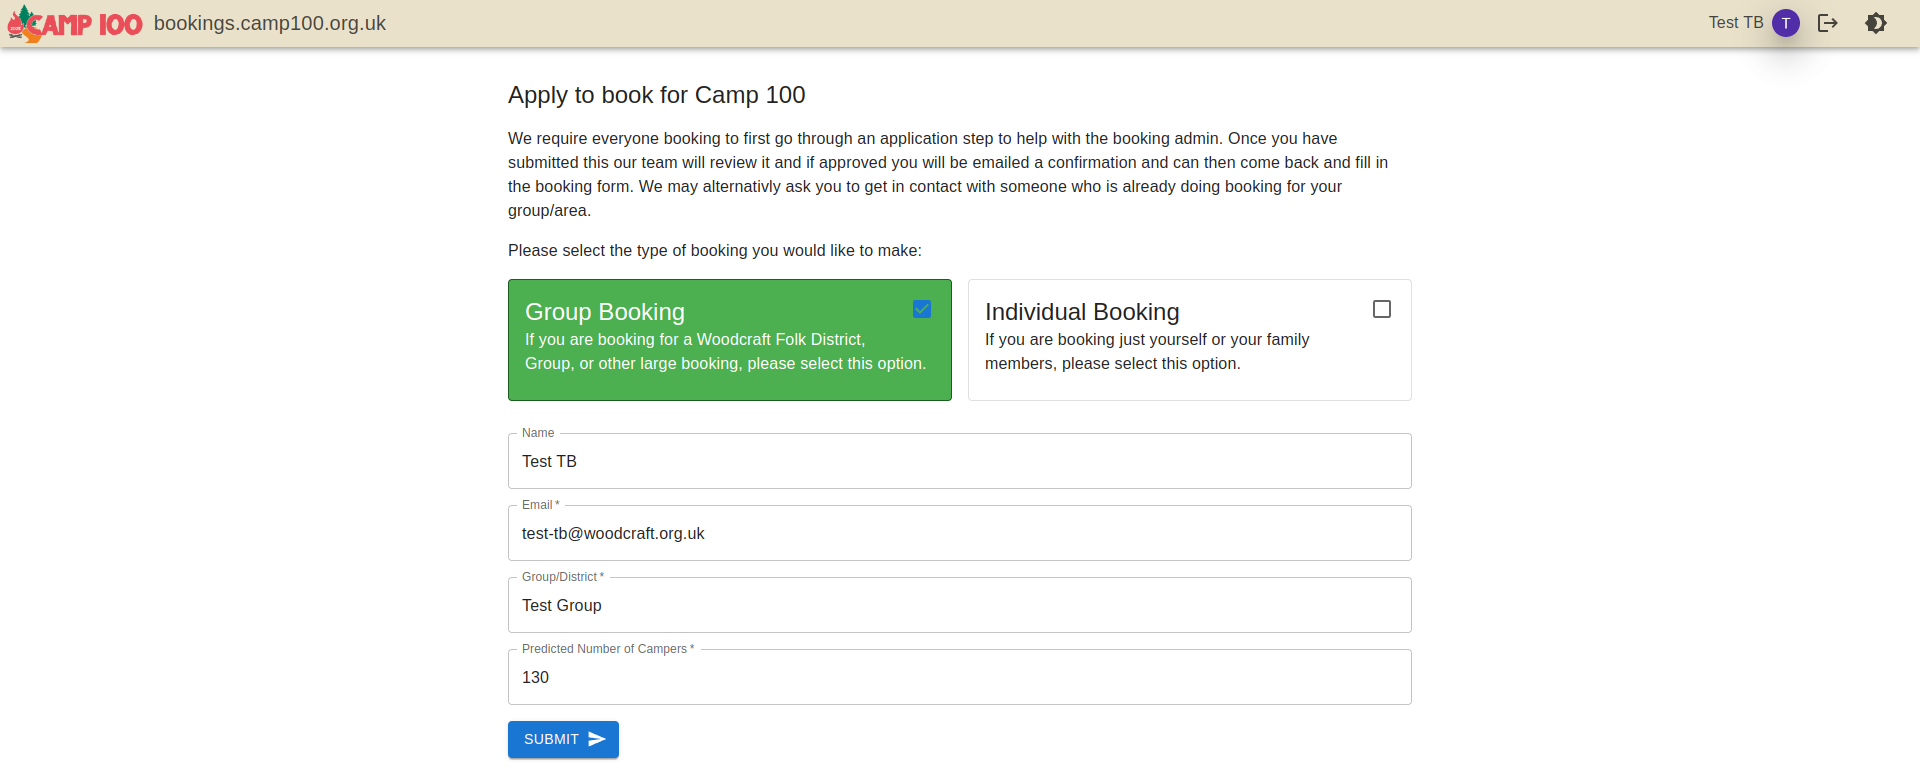
\includegraphics[width=0.9\textwidth]{assets/1-apply.png}
        \caption{Apply To Book page}
    \end{figure}
    \item Your application will now be sent to the Camp 100 team
    \item When your booking has been approved, you will get another email. Continue to \internallink{chap:booking}{Stage 2: Booking}. If from your application it seems like someone else from the same group has already applied to book, we may get in touch to say you should speak to them rather than approving you to book separately.
\end{enumerate}



\chapter{Stage 2: Booking}
\label{chap:booking}

To start in this section, you must have been approved to book. If you are unsure of what that means, see \internallink{chap:apply}{Stage 1: Apply to Book}.

The booking system is set up to be a `live' system. To make it as easy as possible for group leaders we advise that you add people as soon as possible (even whilst your local district/group booking process is still open), as this will spread out the time filling in the information as well as give the Camp 100 team a good idea about numbers. Should you wish you can put in placeholders, e.g `elfin 1', `pioneer 2', until you're clearer on who exactly is coming.

\begin{enumerate}
    \item Go to the \href{https://bookings.camp100.org.uk}{Camp 100 Booking System}
    \item Click `login to book' and ensure you login using the same service which you did last time (this is really important as otherwise, you'll have to apply to book again).
    \begin{figure}[H]
        \centering
        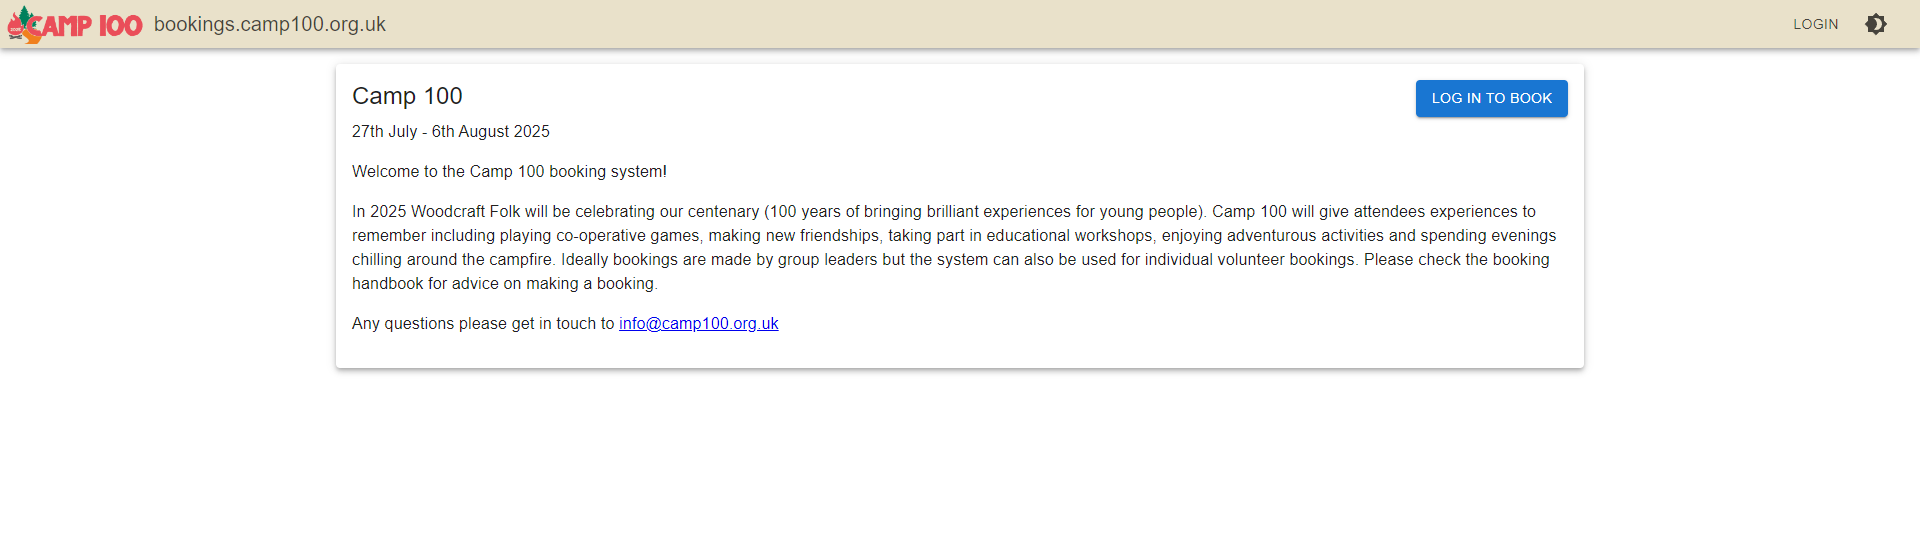
\includegraphics[width=0.9\textwidth]{assets/2-home-prelogin.png}
        \caption{Booking System Homepage}
    \end{figure}
    \item You will now be redirected back to the home page. Click Book.
    \begin{figure}[H]
        \centering
        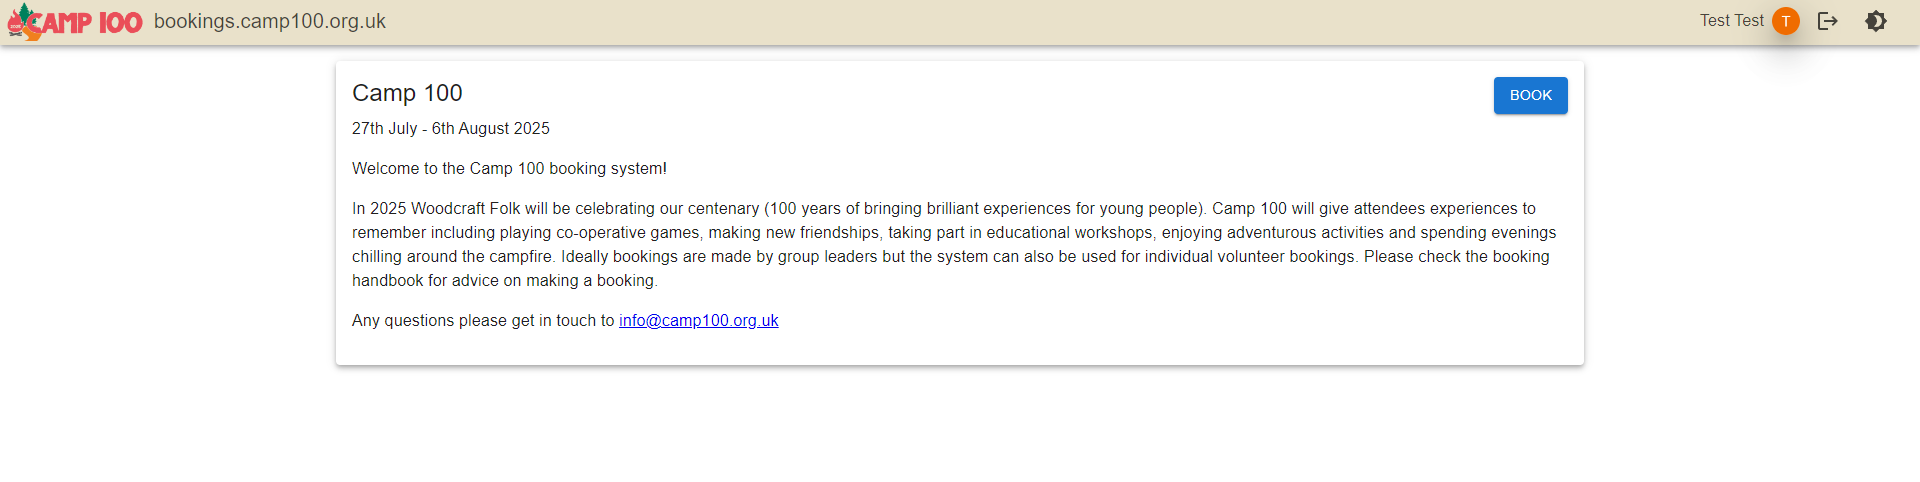
\includegraphics[width=0.9\textwidth]{assets/2-home-loggedin.png}
        \caption{Homepage showing the `Book' button}
    \end{figure}
    \item Now you will need to enter some details about the booking. Enter this information in the text boxes provided. You have the option to add `Extra Contacts' these should be volunteers who are part of your booking and the Camp 100 team can contact everyone on this list and yourself about the camp.
    \item Scroll down to Campers.
    \item We have added an option to complete the booking forms in a spreadsheet rather than using individual forms on the system for each camper. You need to choose whether you want to input the details through a google spreadsheet \textbf{OR} complete the booking using the forms on the booking system. 
    
    If you are \textbf{NOT} using the spreadsheet option skip to \internallink{manual-import}{Step \ref*{manual-import}}

    Spreadsheet instructions:
    \begin{enumerate}
        \item We can create a Google Sheet to fill in and then import the data. This may be easier for larger groups. Clicking the button `create sheet' will create a Google Sheet and share it with the email you have provided. The spreadsheet will ask for the same information as the booking system. 
        
        \textbf{NOTE: Importing from the spreadsheet will overwrite any data you have already entered into the booking system forms so it is important to choose which method you are using.}
        \begin{figure}[H]
            \centering
            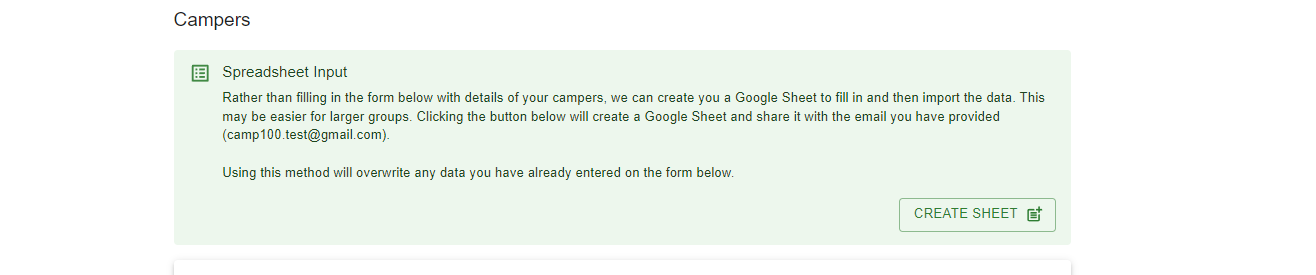
\includegraphics[width=0.9\textwidth]{assets/2-spreadsheet-option.png}
            \caption{Create Sheet button}
        \end{figure}
        \item Once you have created the spreadsheet you will receive an email with a link to the sheet to the email address that you booked with. To access the spreadsheet you will need to have a google account (you can create a google account even without a gmail email address, find support here - \href{https://support.google.com/accounts/answer/27441?hl=en}{support.google.com/accounts/answer/27441?hl=en} ) 
        \item Once you have received the email you can follow the link to open the google spreadsheet
         \begin{figure}[H]
            \centering
            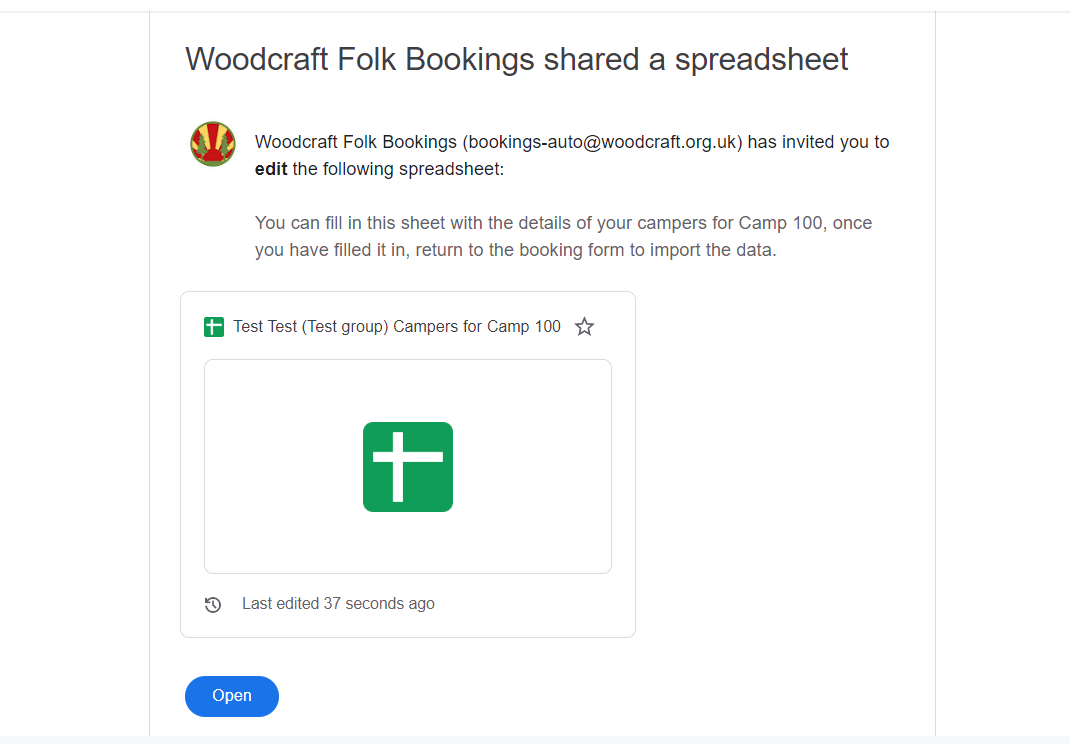
\includegraphics[width=0.6\textwidth]{assets/2-spreadsheet-email.png}
            \caption{Email showing the Shared Spreadsheet}
        \end{figure}
        \item When you open the spreadsheet you will see the same fields as in the booking system forms. We advise that you share the \internallink{chap:template-booking-form}{example consent form} at the end of this guide with parents/carers from your group and use the information to input each camper's data into the spreadsheet. We will need an email address for every camper, if the camper is under 16 this should be the email of a parent or guardian and for over 16s a personal email address where possible. We will use this information to update campers/their parent or guardian with key info and verify Woodcraft Folk membership.
        \begin{figure}[H]
            \centering
            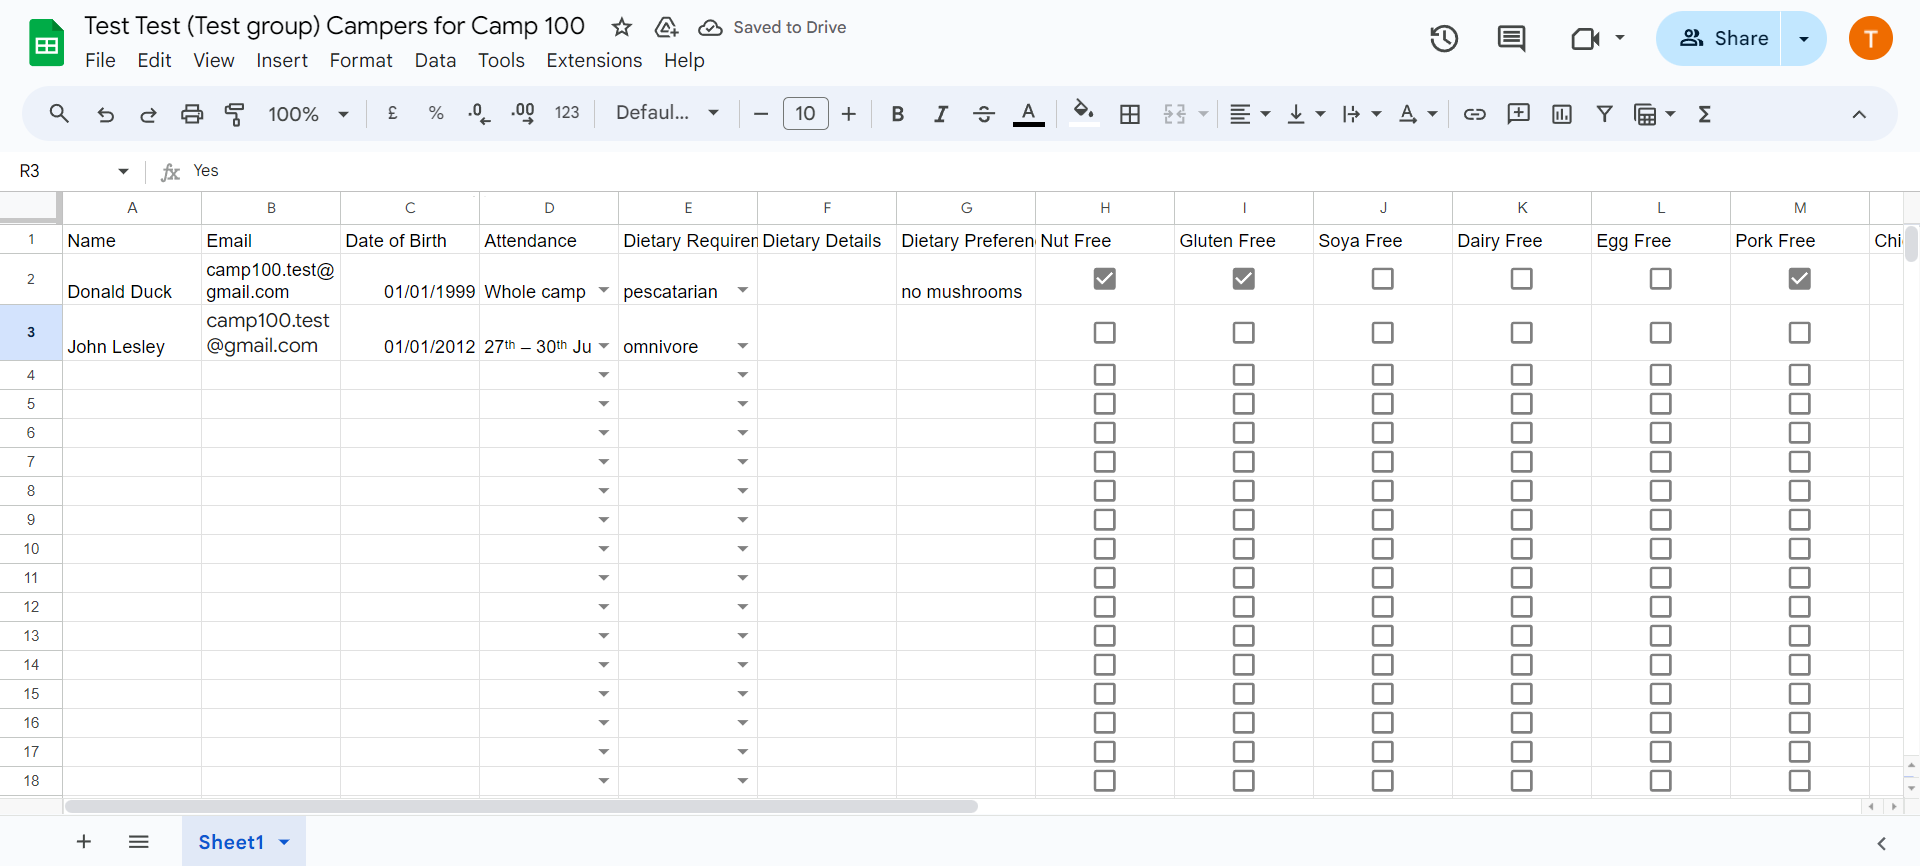
\includegraphics[width=0.9\textwidth]{assets/2-spreadsheet.png}
            \caption{Spreadsheet showing example campers information}
        \end{figure}
        \item You can come back to the spreadsheet and update it, add new campers and remove them anytime before the booking deadline, it will automatically save in the google sheet. You can import the data into the booking system at any time by going back to the booking system and clicking `import data' \textbf{NOTE: Importing from the spreadsheet will overwrite any data you have already entered into the booking system forms.}
        \begin{figure}[H]
            \centering
            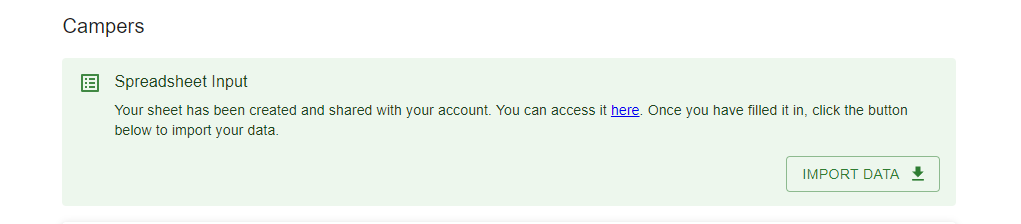
\includegraphics[width=0.9\textwidth]{assets/2-spreadsheet-import.png}
            \caption{`Import Data' button}
        \end{figure}
        \item Once your data has been imported, campers' information will populate the fields in the booking system forms. Campers will be listed on the right hand side of the screen which helps keep a running total of your booking.
        \begin{figure}[H]
            \centering
            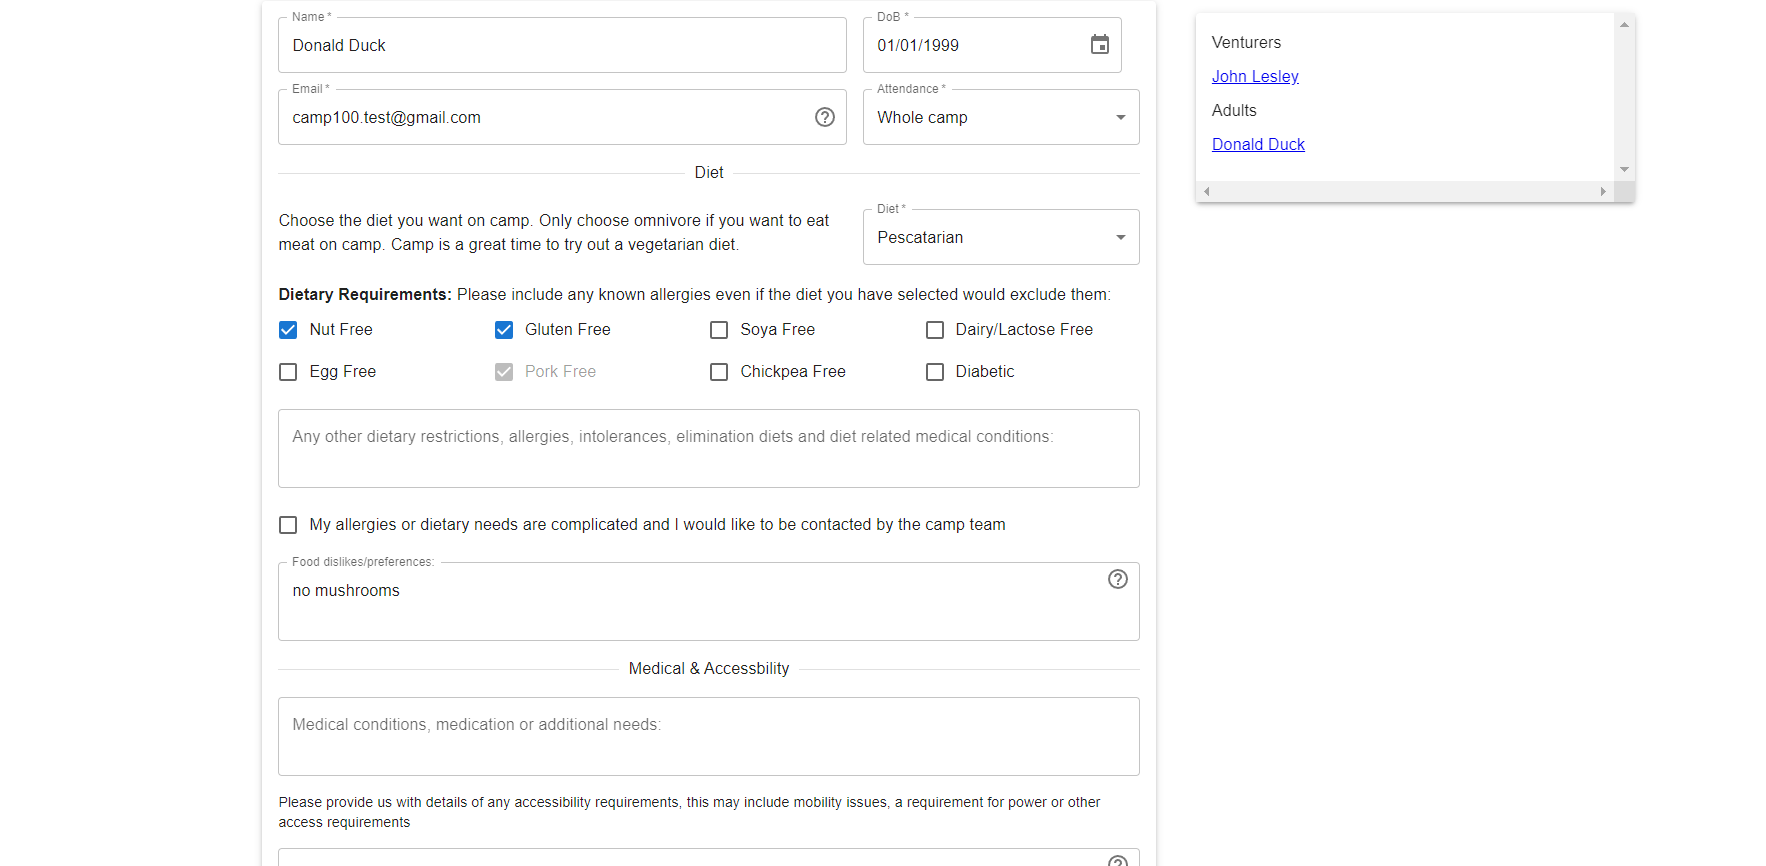
\includegraphics[width=0.9\textwidth]{assets/2-spreadsheet-review.png}
            \caption{Data imported from the spreadsheet show on the booking system}
        \end{figure}
        \item Once you have imported the data from the spreadsheet you need to finish the rest of the form and submit, Skip to \internallink{everyone-steps}{Step \ref*{everyone-steps}} to complete your booking.
    \end{enumerate}
    \item \label{manual-import}  If you are not using the spreadsheet, you will then need to complete the following form for each camper attending. Once added, campers will be listed on the right hand side of the screen which helps keep a running total of your booking. We will need an email address for every camper, if the camper is under 16 this should be the email of a parent or guardian and for over 16s a personal email address where possible. We will use this information to update campers/their parent or guardian with key info and verify Woodcraft Folk membership.
    \begin{figure}[H]
        \centering
        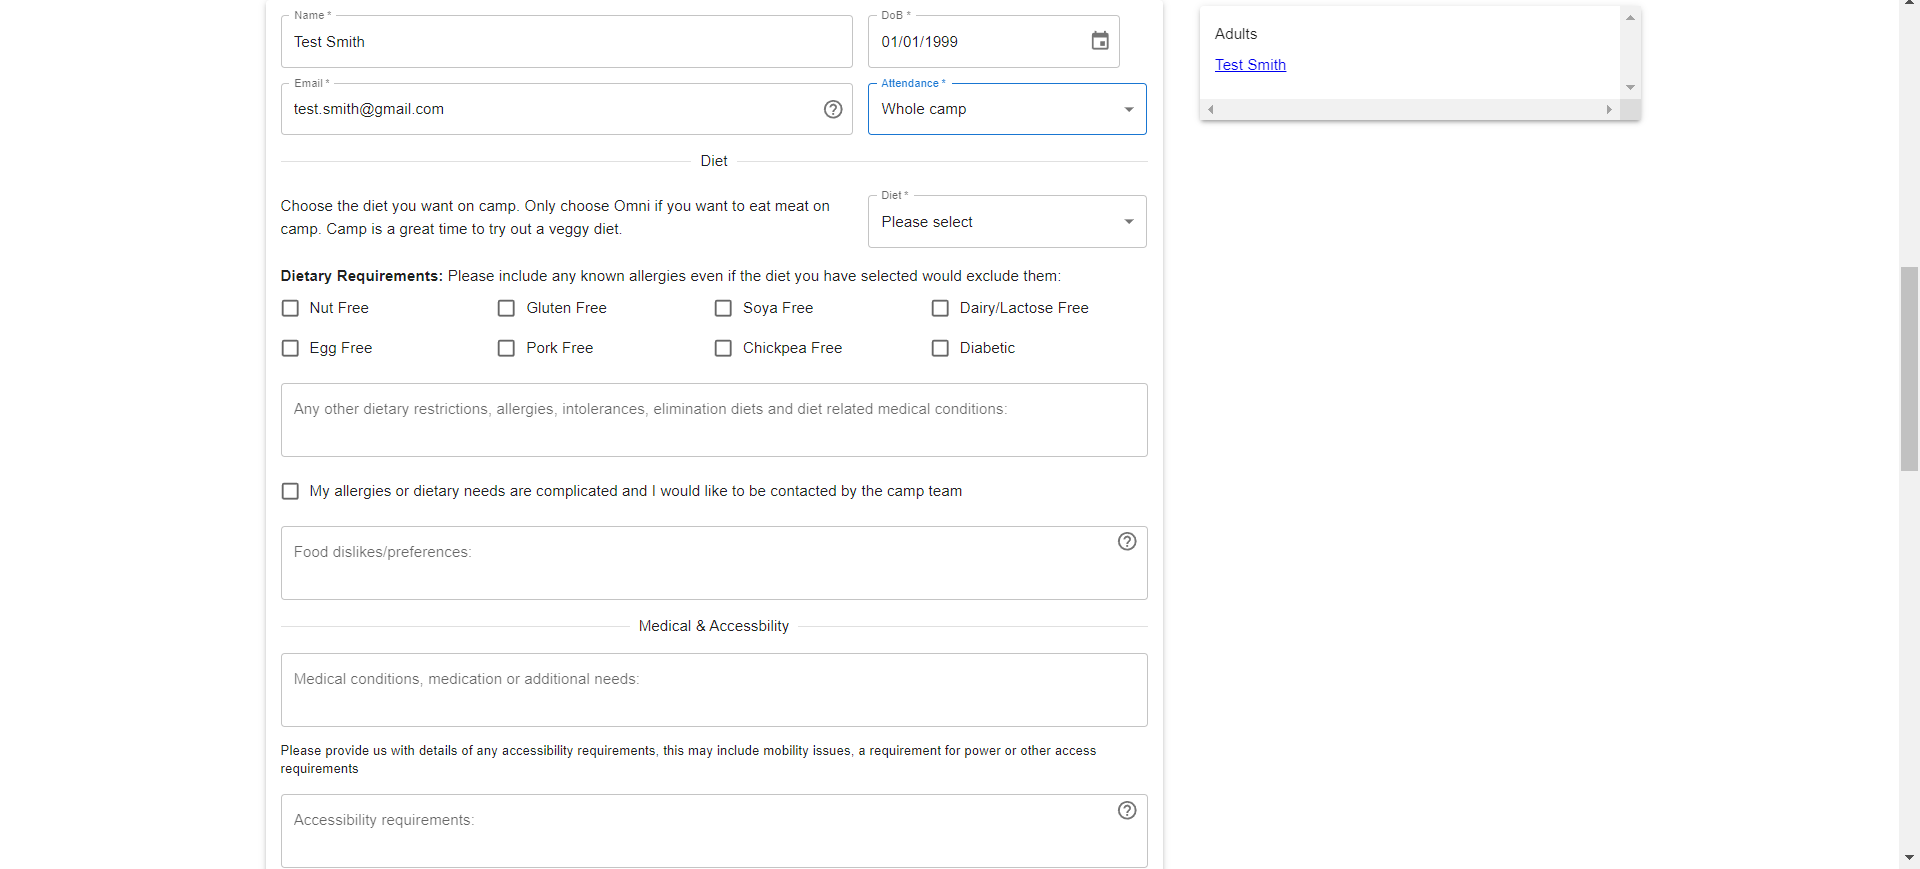
\includegraphics[width=0.9\textwidth]{assets/2-manual-input.png}
        \caption{Manually inputting a participant}
    \end{figure}
    \item To add more campers, click the `Add Person' button. This will add another blank form to complete
    \item To remove a camper, click the orange padlock button to `unlock' the delete button then click the cross button next to it You will then be prompted to confirm that you wish to remove that Participant.
    \begin{figure}[H]
        \centering
        
\includegraphics[width=0.9\textwidth]{assets/2-add-person-button.png}
        \caption{`Add Person' button and orange padlock}
    \end{figure}
    \item \label{everyone-steps}Once you have input information for all your campers scroll down to the heading `Camping'. Here please enter any relevant information about which other groups you would like to camp with, what equipment you have and details of any access needs for your campers. This could include access needs for campers who are yet to book but you anticipate may attend camp. 
    \item Scroll down to Money. Here, you will be given a breakdown of the cost of your group to come to camp, your payment reference which will be C100-XXXXX (which should be used for all payments) and payment instructions. If any of your group apply for an access fund contribution, we will let you know by email whether you are successful and change the amount owed on the system accordingly. See \internallink{chap:payment}{Section \ref*{chap:payment}} for more information on payment. 
    \begin{figure}[H]
        \centering
        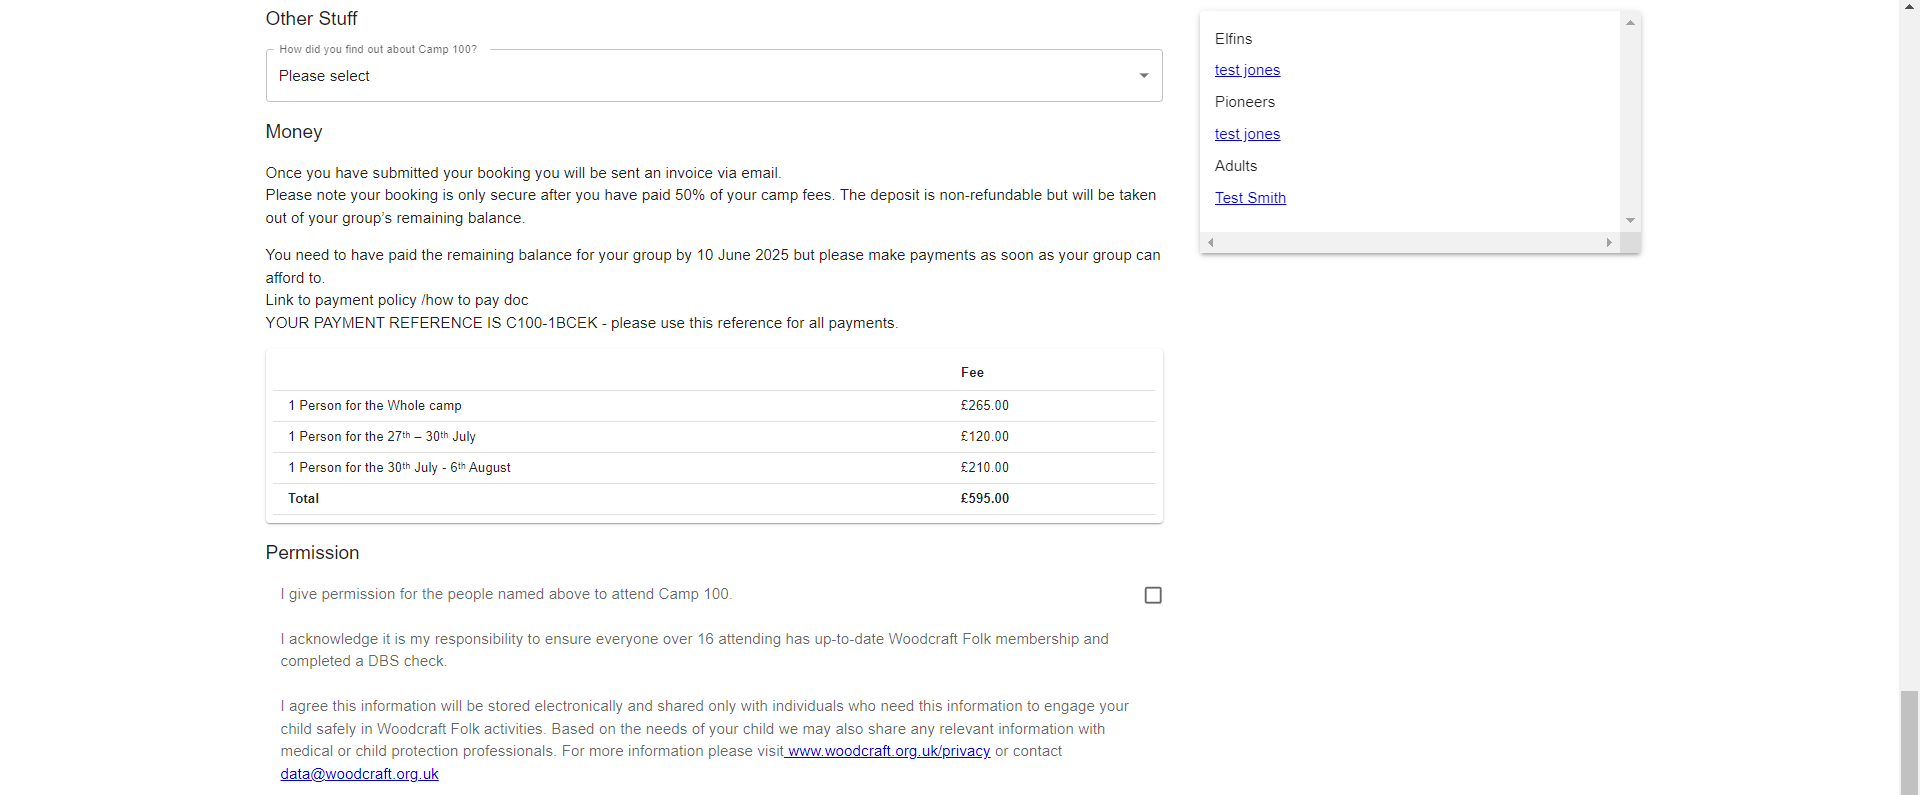
\includegraphics[width=0.9\textwidth]{assets/2-money.png}
        \caption{`Money' Section}
    \end{figure}
    \item Continue scrolling down. For individual bookings, you will need to add the details of someone over 16 who can act as an emergency contact. This is done in the Emergency Contact section.
    \item Give permission for the people to attend and acknowledge responsibility then submit booking. You will be taken to a screen to confirm information about Pricing and an overview of the booking. You will also be sent a confirmation email with an invoice for your booking, this will be amended and resent every time you edit your booking. 
    \begin{figure}[H]
        \centering
        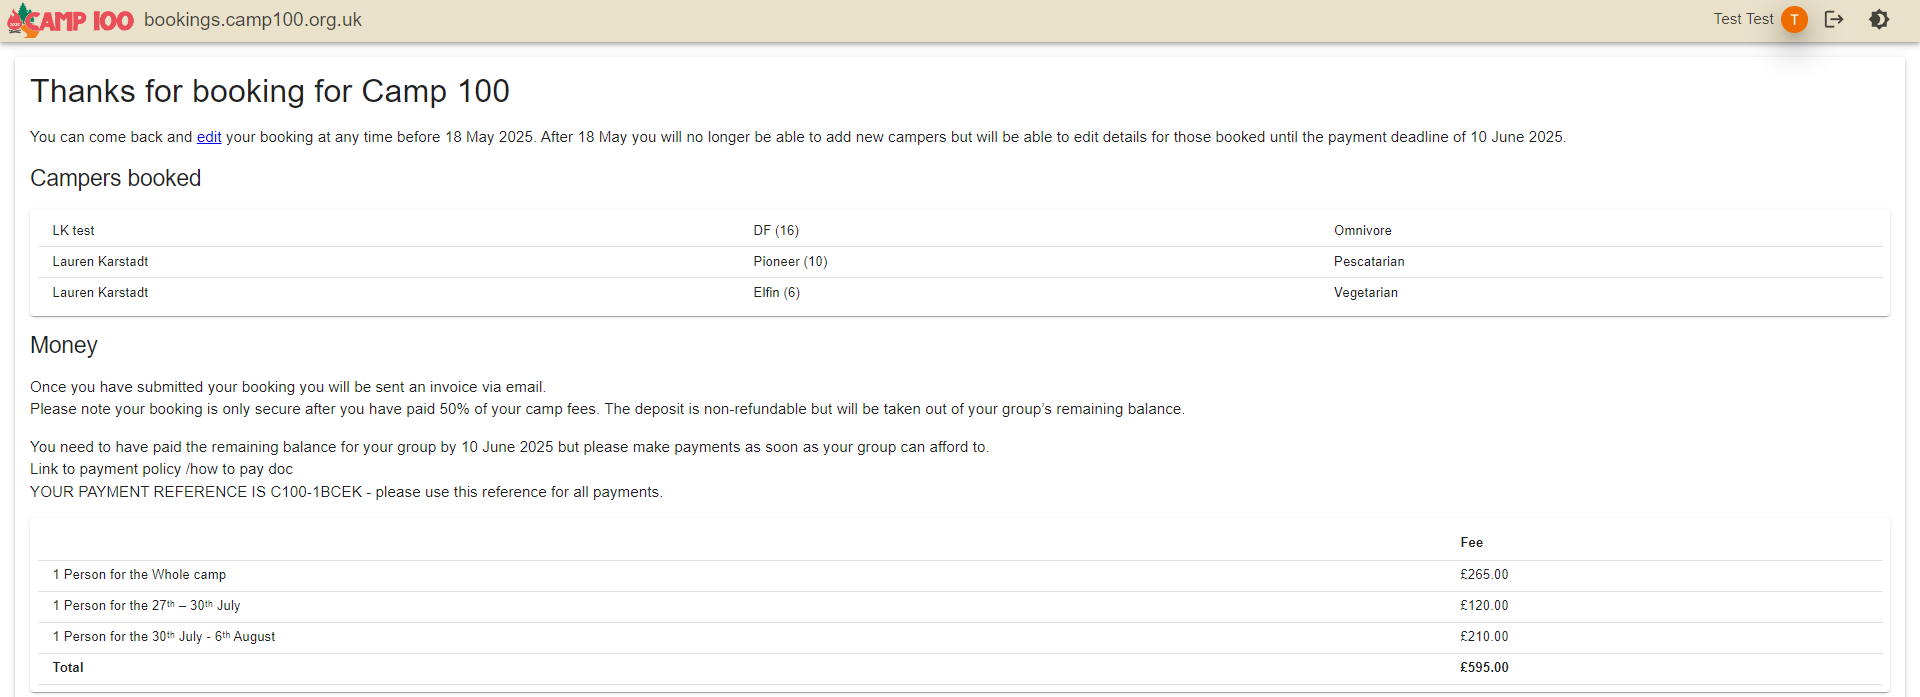
\includegraphics[width=0.9\textwidth]{assets/2-booking-confirmation.png}
        \caption{Booking Confirmation Page}
    \end{figure}
    
\end{enumerate}


\chapter[Stage 3: Edit Bookings]{Stage 3: Edit\\ Booking}
\label{chap:edit}

It is understandable that you will want to add more information or more people to your booking in the build up to Camp 100 

You can edit your booking as many times as you wish up to \textbf{18 May 2025}. After this date you will not be able to add new campers but you may continue to edit your booking if anything changes, although we cannot guarantee being able to change anything at our end or being able to give refunds after this point. The final payment deadline for Camp 100 is 10 June 2025, after this date you will need to speak to Woodcraft Folk staff to edit your booking. 
\begin{enumerate}
    \item Go to the \href{https://bookings.camp100.org.uk}{Camp 100 Booking System}
    \item Click login. Ensure you use the same service to login with as you have previously as otherwise you'll have to apply to book again.
    \item The homepage will show you a summary of your booking and payment information.
    \item Click Edit My Booking.
    \item This will take you to the same page as when you were booking and you can edit your Booking in the system. If you are using the spreadsheet method to book, you can update your spreadsheet and add / remove / amend campers at any time before the deadline. Make sure you import data into the booking system so your invoice and payment information will be updated.
    \item When you have finished editing, you will need to re-check the Permission checkbox, then click Submit booking.
    \item When you have submitted your booking, you will be emailed with a summary of changes and an updated invoice.
\end{enumerate}

\chapter{Payment}
\label{chap:payment}

\begin{callout-orange}{Further Information}
The Payment Policy and full How to Pay information can be found on the \href{https://camp100.org.uk}{Camp 100 Website}
\end{callout-orange}

Once you have booked, you will be assigned a booking reference. This will be in the format C100-XXXXX, (where XXXXX will be replaced with a random code). This is used to uniquely identify your booking. You must use it when paying so we are able to identify the money as coming from you and deduct it from your outstanding balance.

\section{UK Payments}

Please transfer all payments into the following account\\
\textbf{Account name:} Woodcraft Folk\\
\textbf{Account number:} 2039 2756\\
\textbf{Sort code:} 60 83 01

Check the unique reference on your Booking confirmation, ie. C100-XXXXX. Please ensure you will use this reference for the deposit and all subsequent payments.

If for any reason you cannot add a reference, please send an email to info@camp100.org.uk and let us know how much you paid, when you paid it and who it was for. We can then match it to your booking and bring your payment record up to date.

\section{International Payments}

Please transfer all payments into the following account:\\
\textbf{Swift Code (BIC):} NWBKGB2L\\
\textbf{IBAN Number:} GB93NWBK60023571418024\\
\textbf{Address of organisation:} \\
Holyoake House, Hanover Street, Manchester, M60 0AS, United Kingdom

Check the unique reference on your Booking confirmation, ie. C100-XXXXX. Please ensure you will use this reference for the deposit and all subsequent payments. 

If for any reason you cannot add a reference, please send an email to info@camp100.org.uk and let us know how much you paid, when you paid it and who it was for. We can then match it to your booking and bring your payment record up to date

\chapter{After the Booking Deadline}
\section{Read Only Booking Data}
After the bookings deadline on the 18th of May, applying to book (stage 1) and booking (stage 2) will continue to work as they did before, however the process for updating your booking will work a bit differently. When you log on you will be presented with a read-only view of your booking. You can use this to double check the information you have provided. 

\begin{figure}[H]
    \centering
    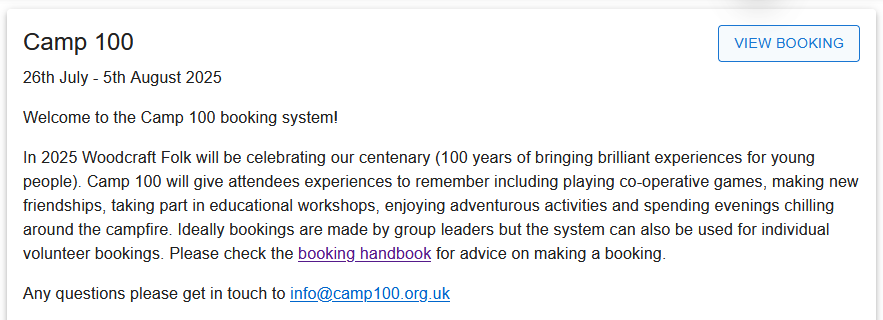
\includegraphics[width=0.9\textwidth]{assets/abd-viewbooking.png}
    \caption{View booking button}
\end{figure}


\begin{figure}[H]
    \centering
    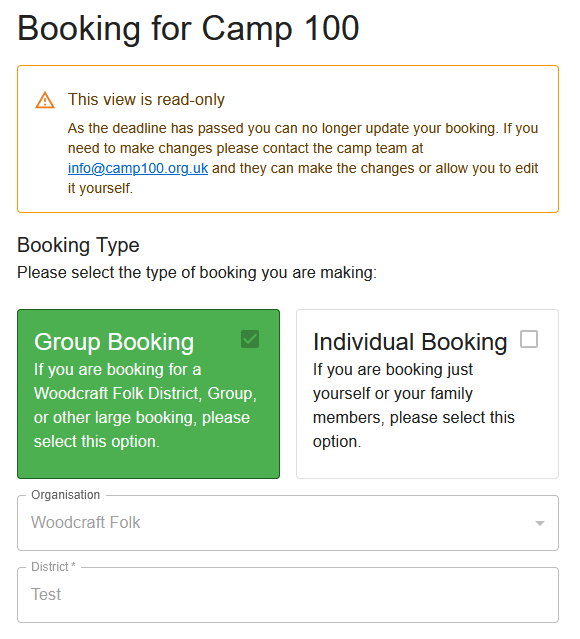
\includegraphics[width=0.4\textwidth]{assets/abd-readonly.png}
    \caption{Read Only notice}
\end{figure}


If you need to make any changes to your booking, please contact the camp team at info@camp100.org.uk and they can either make the changes for you, or for more complicated changes unlock the booking so you can once again edit it yourself.

\section{Late and Cancellation Fees}
Making any changes after the deadline that reduces the fees owed will trigger a cancellation fee of 50\% of the difference between the new fee and the total at the deadline:

\begin{figure}[H]
    \centering
    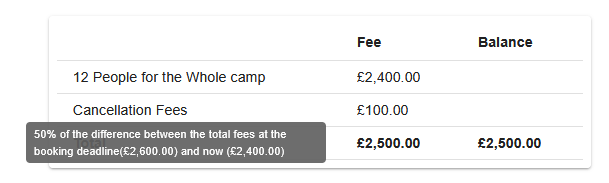
\includegraphics[width=0.9\textwidth]{assets/abd-fees.png}
    \caption{Cancellation fees}
\end{figure}


After the 27th of May, late fees apply and new campers added after this date will cost more:


\begin{table}[H]
    \centering
    {\RaggedRight
    \begin{tabular}{p{0.3\textwidth} p{0.3\textwidth} p{0.3\textwidth}}
    \tablehead{Attendance} & \tablehead{Regular Fee} & \tablehead{After 27 May}\\
    10 days & £265 & £350 \\
    \hline
    7 days & £210 & £285 \\
    \hline
    3 days & £120 & £160\\
    \hline
    \end{tabular}
    } % end of rr     
    \caption{Payment structure including late fees}
    
\end{table}

\chapter{Template Booking Form}
\label{chap:template-booking-form}

A template booking form has been produced which group leaders are able to use to collect information about those in their group before inputting it into the booking System. Some of the information below will be just for district/group reference and not asked for centrally so please keep these forms for information such as in case of emergency and doctor’s details.  It has been included below for reference only, an editable copy is available to \href{https://drive.google.com/file/d/1oSFIkZQxzes3VTi5ZqPHCcAu4DiscvOm/view}{download from here}. 

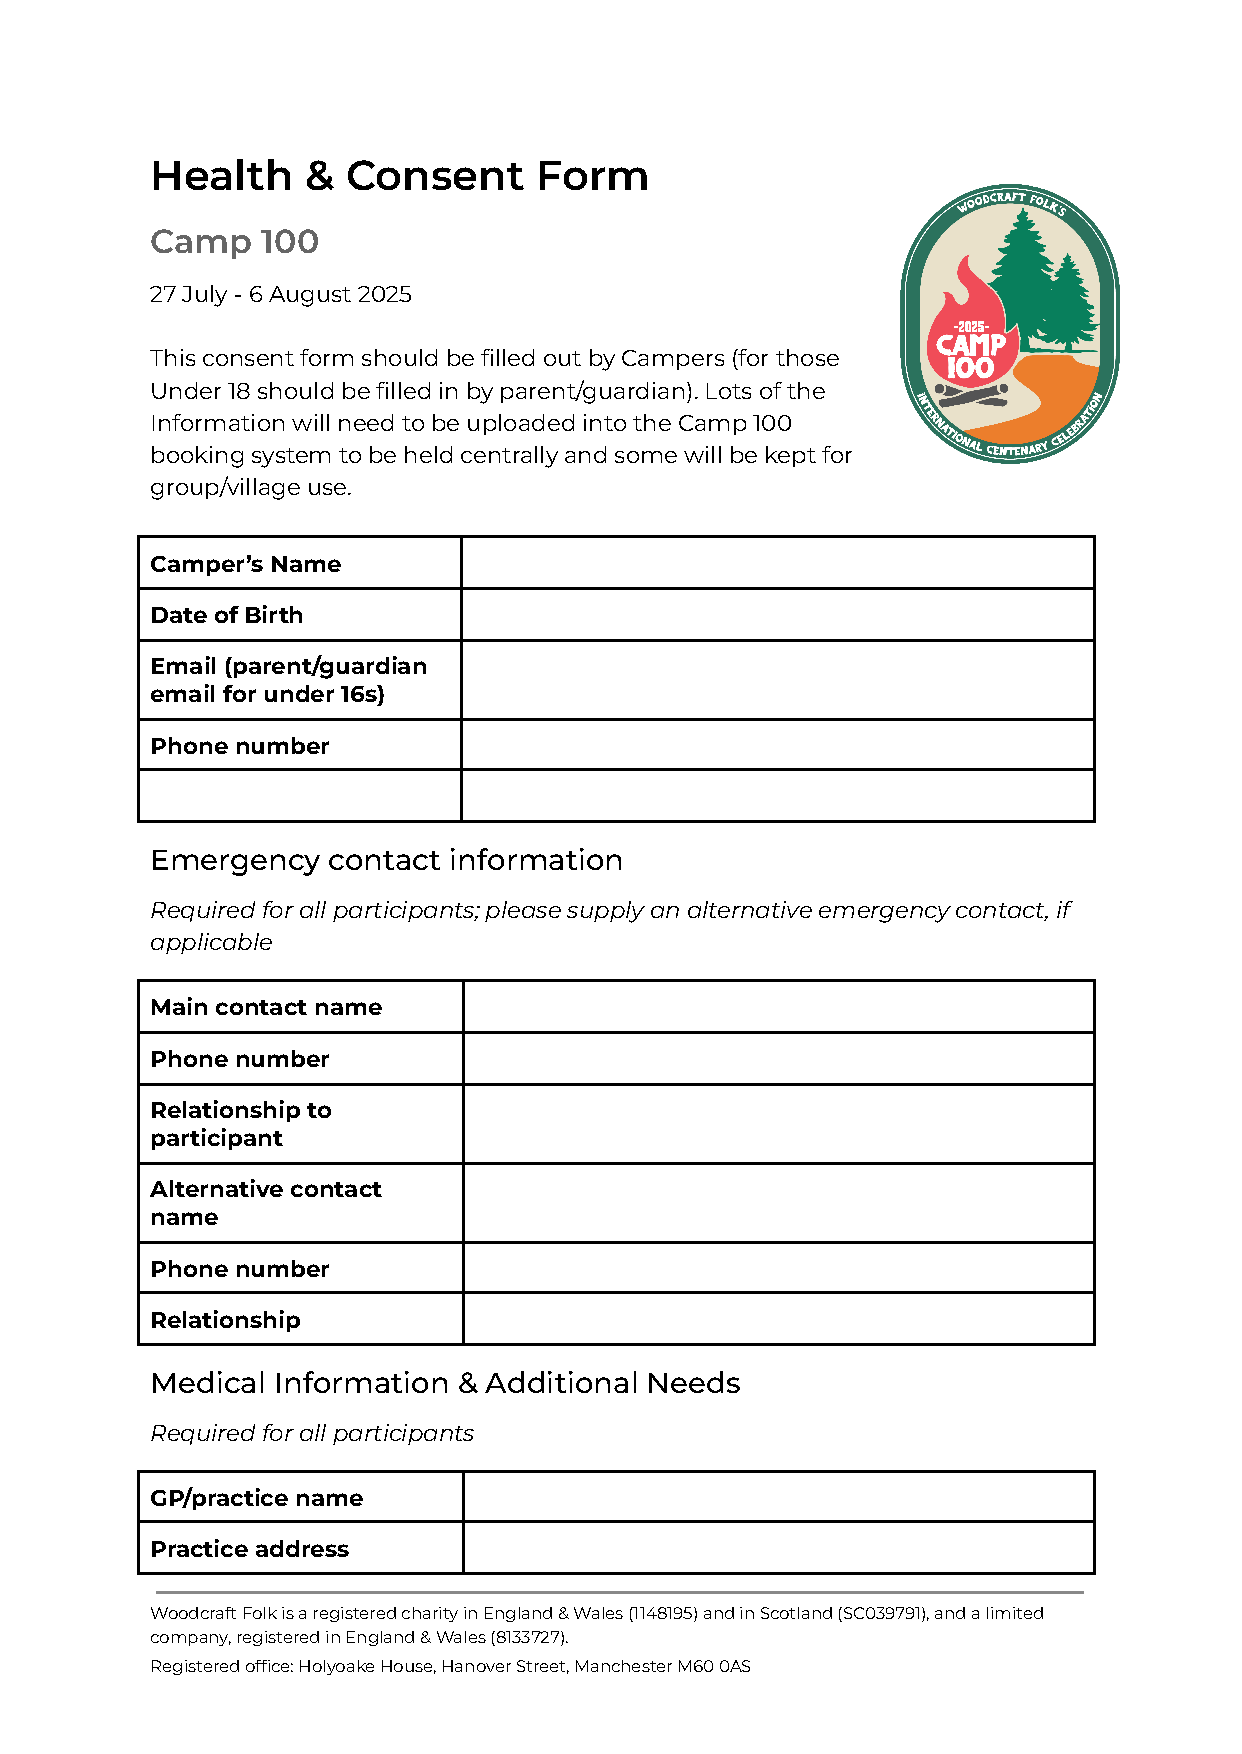
\includepdf[pagecommand={\pagestyle{fancy}}, scale=0.8, pages=-, frame]{assets/template-consent-form.pdf}

\makedocumentbackpage

\end{document}